\begin{evenBlock}{Endzone Soccer (Dribble)}
\textbf{Goal:} Learn to recognize open space and how to attack that open space and beat a defender.  Learn to know when to pass as defensive pressure builds around you.
\begin{minipage}[t]{\linewidth}
    \begin{minipage}{.3\linewidth} % Left column and width
        \centering
        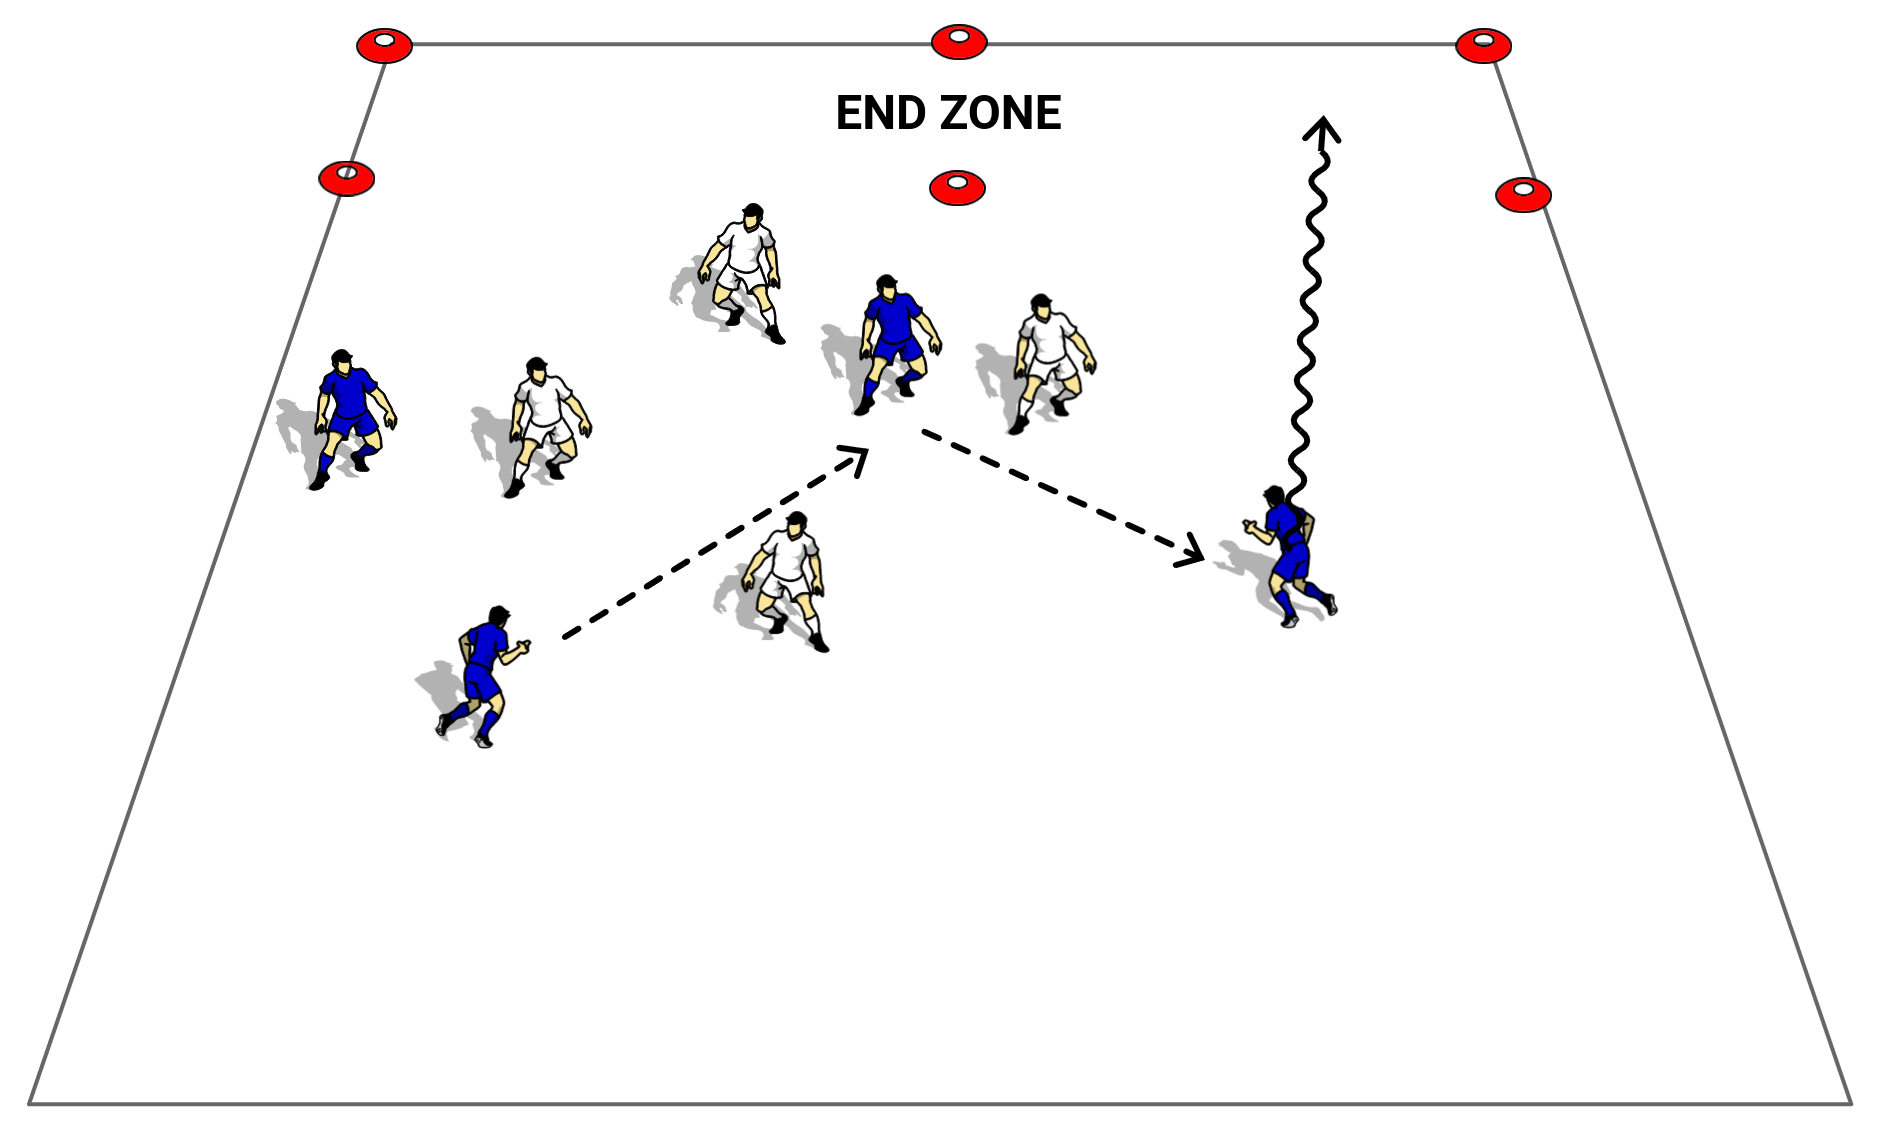
\includegraphics[width=\textwidth]{../img/Trimmed/EndZoneSoccer_DribbleScore}
    \end{minipage}
    \hspace{0.05\linewidth}
    \begin{minipage}{.6\linewidth} % Left column and width
        \textbf{Drill Description:}
        \begin{enumerate}
            \setlength{\itemsep}{0pt}
            \setlength{\parskip}{0pt}
            \setlength{\parsep}{0pt}
            \item 4v4 Small sided activity.
            \item The goal is to dribble the ball into the end zone under control and stop the ball.
            \item Only the person with the ball can enter the end zone unless the defender is backed into the endzone by the attacking player.
            \item Once the ball is stopped in the endzone that team scores and the other team gets the ball at the top.
            \item If the defending team steals the ball they become the attackers but must pass the ball at least once before entering the endzone.
            \item Any out of bounds plays result in the defending team winning the ball, unless the defending team kicks the ball out the back of the end zone.
            \item If the attacking team passes the ball into the endzone the ball is dead and awarded to the defending team.
        \end{enumerate}
    \end{minipage}
\end{minipage}
\raggedright
    \textbf{Coaching Points:}
    \begin{itemize}
        \setlength{\itemsep}{0pt}
        \setlength{\parskip}{0pt}
        \setlength{\parsep}{0pt}
        \item Look to exploit open space in front or behind the defender.
        \item Use and try moves to beat the defender.
        \item Learn how to time these moves, usually they need to happen sooner than one thinks.
        \item Learn to feel the defensive pressure and passing to an open teammate.
        \item Learn to keep your head up and find an open player.

    \end{itemize}

\end{evenBlock}